% Rathmann et al., 2025

\documentclass[tikz,11pt,border=5pt]{standalone}

\usetikzlibrary{arrows.meta}
\usetikzlibrary{fadings}
\usepackage{xcolor}
\definecolor{mybar}{HTML}{1f78b4}

\input{../fonts.tex}

\tikzset{
	every picture/.style={font=\fontsize{10}{10}\selectfont},
	axis/.style={Latex-Latex, very thick},
	tick/.style={dashed, thick}, 
	ticknode/.style={above}, 
	annotate/.style={below, yshift=-0.5em, align=center, fill=white, inner sep=0.15em, font=\fontsize{9.5}{9.5}\selectfont},
}

%%%%%%%%%%%%%%%%

\gdef\L{17.2em}
\gdef\Lm{\L*3/6}
\gdef\dL{\L/6}
\gdef\Lpad{0.025*\dL}

\gdef\Htick{16.3em}

\gdef\dH{0.75em}

\gdef\dyrow{3.25em}
\gdef\dxbar{0.035*\L}

%%%%%%%%%%%%%%%%

\pgfdeclarehorizontalshading{fr}{2cm}{
	color(0cm)=(pgftransparent!0); 
	color(1.5cm)=(pgftransparent!0); 
	color(2cm)=(pgftransparent!100)
}
\pgfdeclarefading{fadeR}{\pgfuseshading{fr}}

\pgfdeclarehorizontalshading{fl}{2cm}{
	color(0cm)=(pgftransparent!100); 
	color(0.5cm)=(pgftransparent!0);
	color(2cm)=(pgftransparent!0)
}
\pgfdeclarefading{fadeL}{\pgfuseshading{fl}}

\begin{document}

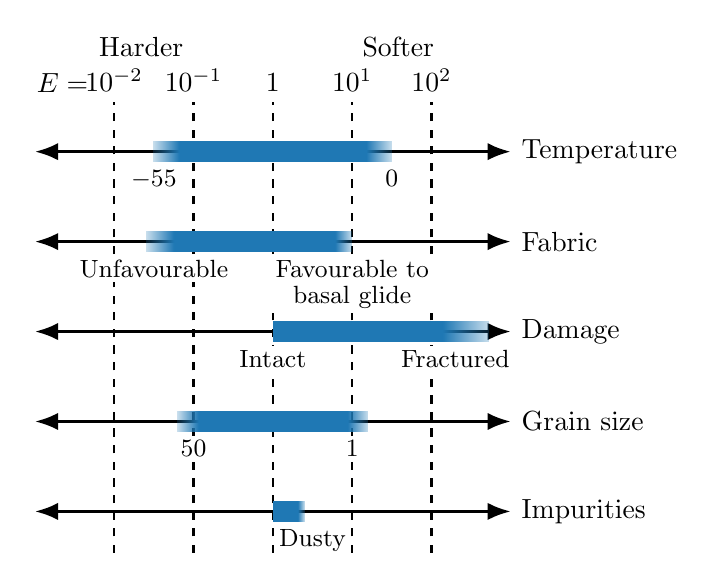
\begin{tikzpicture}[]

\begin{scope}[shift={(0,-1.5em)}]
\node[ticknode,xshift=1em] at (\L*0/6,\Htick) {$E=$};
\draw[tick] (\L*1/6,0) -- ++(0,\Htick) node[ticknode] {$10^{-2}$};
\draw[tick] (\L*2/6,0) -- ++(0,\Htick) node[ticknode] {$10^{-1}$} node[left, yshift=2em] {Harder};
\draw[tick] (\L*3/6,0) -- ++(0,\Htick) node[ticknode] {$1$};
\draw[tick] (\L*4/6,0) -- ++(0,\Htick) node[ticknode] {$10^{1}$} node[right, yshift=2em] {Softer};
\draw[tick] (\L*5/6,0) -- ++(0,\Htick) node[ticknode] {$10^{2}$};

\end{scope}

\begin{scope}[shift={(0,4*\dyrow)}]
	\draw[axis] (0,0) -- ++(\L,0) node[right] {Temperature};
	\fill[mybar, path fading=fadeR] (\Lm,-\dH/2) rectangle ++(1.5*\dL,\dH);
	\fill[mybar, path fading=fadeL] (\Lm+\Lpad,-\dH/2) rectangle ++({-1.5*(\dL+\Lpad)},\dH);
	\node[annotate] at (1.5*\dL,0) {$\SI{-55}{\degreeCelsius}$};
	\node[annotate] at (4.5*\dL,0) {$\SI{0}{\degreeCelsius}$};
\end{scope}

\begin{scope}[shift={(0,3*\dyrow)}]
	\draw[axis] (0,0) -- ++(\L,0) node[right] {Fabric};
	\fill[mybar, path fading=fadeR] (\Lm,-\dH/2) rectangle ++( 1*\dL,\dH); 
	\fill[mybar, path fading=fadeL] (\Lm+\Lpad,-\dH/2) rectangle ++(-1.6*\dL-\Lpad,\dH); 
	\node[annotate] at (\Lm+\dL,0) {Favourable to\\basal glide};
    \node[annotate] at (\Lm-1.5*\dL,0) {Unfavourable};
\end{scope}

\begin{scope}[shift={(0,2*\dyrow)}]
	\draw[axis] (0,0) -- ++(\L,0) node[right] {Damage};
	\fill[mybar, path fading=fadeR] (\Lm,-\dH/2) rectangle ++(2.73*\dL,\dH); 
	\node[annotate] at (\L*3/6,0) {Intact};
	\node[annotate] at (\L*5.3/6,0) {Fractured};
\end{scope}

\begin{scope}[shift={(0,1*\dyrow)}]
	\draw[axis] (0,0) -- ++(\L,0) node[right] {Grain size};
	\fill[mybar, path fading=fadeR] (\Lm,-\dH/2)       rectangle ++(1.2*\dL,\dH);
	\fill[mybar, path fading=fadeL] (\Lm+\Lpad,-\dH/2) rectangle ++({-1.2*(\dL+\Lpad)},\dH);
	\node[annotate] at (2*\dL,0) {$\SI{50}{\milli\metre}$};
	\node[annotate] at (4*\dL,0) {$\SI{1}{\milli\metre}$};
\end{scope}

\begin{scope}[shift={(0,0*\dyrow)}]
	\draw[axis] (0,0) -- ++(\L,0) node[right] {Impurities};
	\fill[mybar, path fading=fadeR] (\Lm,-\dH/2) rectangle ++(0.4*\dL,\dH); 
	\node[annotate] at (\Lm+0.5*\dL,0) {Dusty};
\end{scope}

\end{tikzpicture}

\end{document}